\documentclass{beamer}
\usepackage{hyperref}
\usepackage{graphicx}

\begin{document}
\section{Topological Maps}
\begin{frame}{Topolgical Maps}
 \textbf{Topological maps}: describe the environment as a graph that connectecs specific locations in the world and represents them as vertices.
 \begin{enumerate}
 	\item Because metric representations cost too much memory to maintain in the long run.
 	\item Easy to understand for humans.
 	\item The nodes on the graphs are landmarks or features of the environment. The edges are paths between the different nodes. 
 	\item Landmarks can be artificial or natural.
 	\item Landmarks can look the same so you need to make sure you dont use two or more nodes to represent the same landmark.
 \end{enumerate}
\end{frame}

\begin{frame}{Marker based Exploration}
 \begin{enumerate}
 	\item No prior information about the environment available.
 	\item Can be extended by enumerating the edges incident to the node entered. Edge you traveled along is 0 and enumerate clockwise. This enumeration is local cause it depends on the edge the robot moved over.
 	\item Landmarks aren't distinguishable from eachother.
 	\item The robot needs to have something to mark where it has already been.(spray paint, bread crumbs)
 	\item Use unique marks which it can pick up, drop and recognize.
 \end{enumerate}
 
\end{frame} 

\begin{frame}{Marker based exploration algorithm}
	\begin{enumerate}
		\item Builds up the known graph by traveling along the incident edges.
		\item $v_{i}$ is the node where the robot is currently at. $v_{j}$ is the node where the robot is moving to. $E_{i,j}$ is the edge between the 2 nodes.
		\item Transition function need to follow these properties. If $(v_{i},E_{i,j},r) = v_{j} $ and $(v_{j},E_{i,j},s) = v_{k} $, then $v_{j},E_{i,j},-s) = v_{i}$
		\item Moves are invertible and can be retraced.
		\item $t \neq -s$ then $v_{j},E_{i,j},-s) = v_{i}$ and  $(v_{j},E_{i,k},s) = v_{j}$ are not valid. To avoid redundant and degenerate paths.
	\end{enumerate}
\end{frame}

\begin{frame}{Marker based exploration algorithm(2)}
	\textbf{Operations for the robot}
	\begin{enumerate}
		\item r stands for move along the given edge.
		\item Each marker can be in 3 different states[pickup,putdown,null]
		\item Marker based perception: At each vertex the robot can see two things [present, not-present]
	\end{enumerate}
	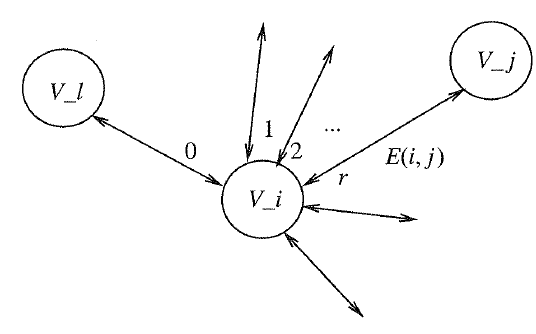
\includegraphics[scale= 0.5]{edgeordering.png}
\end{frame}

\begin{frame}{Marker based exploration algorithm (3)}
	\textbf{Operations for the robot}
	\begin{enumerate}
		\item Robot can determine the relative posotions of the edges by enumerating the edges like said before. 
		\item Entering the same vertex from a different edge gives 2 different ordering. The robot needs to make a global ordering. 
		\item Subgraph S for explored edges and U for unexplored are incident to unknow nodes.
		\item First validate all explored nodes. Make sure there aren't any doubles by looking for markers.
		\item	If there is no marker found at a certain node v add it the subgraph S and add the edge which was taken aswell.
		\item Enumerate all edges incident to the new node and add them to U. 
		\item Do this till subgraph U is empty.
	\end{enumerate}
\end{frame}

\begin{frame}{Example}
	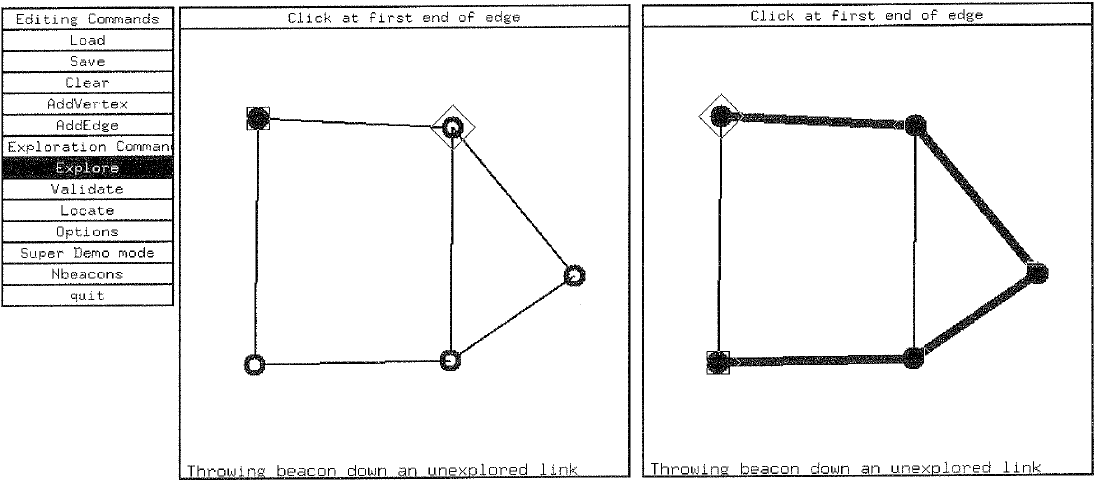
\includegraphics[scale =0.3]{voorbeeld.png}
\end{frame}

\section{Multiple Robots}
\begin{frame}{Multiple Robots}
	\textbf{Why would you use multiple Robots}
	\begin{enumerate}
		\item \textbf{Improved Robustness}: A multirobot can ,in principle, keep functioning even if one indiviudual robots dail completely. 
		\item \textbf{Improved effiency}: It is possible for a group of robots to accomplish a search or exploration task faster than an equivalent single robot.
		\item \textbf{Alternative Algorithms}: For some tasks, the availability of multiple robots allows feadible or guaranteed algorithms to be implemented when no such algorithm is 		available for a single robot system. 
	\end{enumerate} 
\end{frame}

\begin{frame}{Multi Robots in Practice}
	\textbf{Problems}
	\begin{enumerate}
		\item \textbf{Where are teh other robots?}: Rendezvous with other robots
		\item \textbf{Partitioning}: Finding a good way to distribute the work amongst the robots.
		\item \textbf{Multi-robot planning}: Prevent the trajectories of the robots to collide. 
		\item \textbf{Merging the data from the indivual team}:
	\end{enumerate}	
\end{frame}

\begin{frame}{Rendezvous}
	\textbf{Rendezvous}: Is a having two or more robots meet at an appointed place and time. 
	\begin{enumerate}
		\item Rendezvous is needed for robots that can only communicate in close proximities, but may also be needed to exchange objects between robots.
		\item When Multiple robots try to complete a task collaborotavely without prior knowledge. They need to to exchange information while they are still working at the task at hand.  
		\item	 If they dont meet they cannot benefit from what others have already learned. 
	\end{enumerate}
\end{frame}

\begin{frame}{Too many Rendezvous}
	\textbf{Problems}:Robots mustn't devote too much energy to rendezvous
		\begin{enumerate}			
			\item The extent to which the two robots agree on their perceptions of the environment. What is the difference 
			\item The degree of synchornization of the robots can attain expressed as the likelihood that an appointed rendezvous at a common location will fail owning to a failure to arrive at the same time
			\item The extent Of the commonality between the region of space the robots have explored.
		\end{enumerate}
	\textbf{There are many different rendezvous algorithms}
	\begin{enumerate}
		\item \textbf{plan based}: 
		\item \textbf{stochastic algorithmes}: One stationary and one seeks or Randomly visit rendezvous points which are points or interest.
	\end{enumerate}
\end{frame}

\begin{frame}{Map fusion}
	\textbf{Map fusion}: is needed when the problem doesn't involve foraging.
	\begin{enumerate}
		\item Is needed to make the collaborative effort worthwhile.
		\item Complexity of the map-merging depends on the , Odemetry error, the fidelity of the sensing used. and the richness of the evironment.
		\item Fusing maps using cross correlation depends on teh fact that the individual maps overlap "sufficiently'.
		\item Done by rotation and translating of the given maps.
	\end{enumerate}	
\end{frame}

\begin{frame}{Exploration with Multiple robots}
	\begin{enumerate}
		\item Robots are only allowed to commnicate when they are in the same node.
		\item Split all the work between all the robots and have them explore their own part of the graph.
		\�tem Plan rendezvous, to harmonize the information they got till then and make a single consistent representation of the environment they are in.
		\item Redevide the work and repeat this till everything is known. 
	\end{enumerate}
\end{frame}
\begin{frame}

	\url{http://www.csupomona.edu/~ftang/courses/CS499/notes/navigation3.pdf }
\end{frame}

\end{document}